Normalizing flows, diffusion models and generative flow networks (GFlowNets) are proposed as samplers of Boltzmann distributions $p(x)\propto e^{-\beta U(x)}$ for molecules and materials \citep{noe2019boltzmann,hoogeboom2022edm,satorras2021egnn,lipman2023flowmatching}. The partition function $Z$ of such systems is unknown, so a learned sampler is usually judged by statistics of its own importance weights: the effective sample size (ESS), the Pareto $\hat k$, and delta-method intervals for the free energy.

These statistics share a critical failure mode: they are computed exclusively from configurations the sampler proposed, so a basin it never proposes leaves no trace in them. Section~\ref{sec:theory} formalizes this diagnostic blindness: conditioned on never visiting a basin of Boltzmann mass $\alpha$, the importance weights follow the law of the problem with that basin deleted. As a result, the free-energy estimate is shifted by $-\beta^{-1}\log(1-\alpha)$ while the ESS remains high and nominal confidence intervals shrink at rate $O(M^{-1/2})$ around the wrong value, so coverage falls toward 0\% for as long as the basin stays unvisited (Figure~\ref{fig:molecular_pathology}). While support coverage is an elementary requirement of importance sampling, modern evaluation culture has overlooked a critical consequence: self-reported diagnostics falsely reward mode collapse with high confidence, reporting near-optimal ESS and contracting intervals precisely when macroscopic states are omitted.

\begin{figure}[t]
\centering
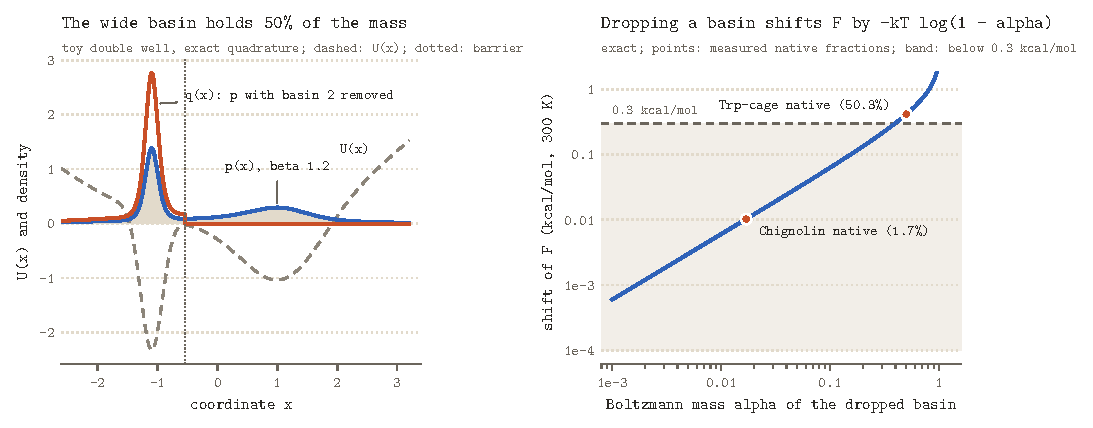
\includegraphics[width=\linewidth]{figures/fig_molecular_pathology.pdf}
\caption{Left: the toy double well of Section~\ref{sec:bidirectional} at $\beta=1.2$. The narrow basin is the energy minimum, but the wide basin holds $\vtoyMassTwo\%$ of the Boltzmann mass (exact quadrature). Shaded: $p$. $q$ is $p$ with the wide basin removed. Right: shift of the free energy at 300\,K when a basin of mass $\alpha$ is never proposed, $-k_BT\log(1-\alpha)$ (exact). Points mark native-basin fractions; shaded: shifts below 0.3\,kcal/mol.}
\label{fig:molecular_pathology}
\end{figure}

To determine how this pathology manifests across physical systems, we organize our evaluation into three tiers:
\begin{enumerate}
\item \textbf{Exact empirical audit on disordered systems (Section~\ref{sec:benchmarks}):} Spin glasses feature frustrated, multi-basin landscapes where ground-truth partition functions can be enumerated exactly up to $n=28$ spins. On these references, masked diffusion and GFlowNets exhibit severe calibration collapse, covering exact values in only $\vcovDiffTwo\%$ and $\vcovGFNTwo\%$ of runs at $\beta=2$. In contrast, classical thermal estimators and normalized autoregressive networks (VAN-MADE) remain calibrated near 95\%.
\item \textbf{Continuous neural molecular sampler (Section~\ref{sec:bidirectional}):} On an analytic surrogate of the alanine dipeptide Ramachandran surface, a RealNVP flow trained by reverse KL drops the $C_{7\rm ax}$ basin ($\valaAlpha\%$ mass), yet reports a median ESS of $\valaESS\%$ while nominal interval coverage collapses to $\valaCov\%$. An independent reverse check immediately flags the omission ($G_{\rm rev} = \valaGrev$\,nats).
\item \textbf{Macromolecular landscape sizing (Section~\ref{sec:molecular_case}):} We size the bound in kcal/mol with all-atom simulations of chignolin and Trp-cage and a Langevin sweep of the LJ$_{38}$ cluster. Omitting the Trp-cage native basin would shift $F$ by $\vtrpBias$\,kcal/mol at the fraction measured in our run; single trajectories also show the blind spot themselves, since they report nothing about basins they have not reached.
\end{enumerate}

\paragraph{Contributions.} (i) A formal proposition proving that self-normalized diagnostics and confidence intervals are blind to unvisited Boltzmann mass (Section~\ref{sec:theory}). (ii) A combinatorial benchmark comparing learned versus classical samplers against exact ground truth (Section~\ref{sec:benchmarks}). (iii) A reverse check that flags dropped basins in an exact toy and in flows on model landscapes, with its limits (Section~\ref{sec:bidirectional}). (iv) Molecular simulations that size the shift in kcal/mol and show the single-trajectory analogue (Section~\ref{sec:molecular_case}).